\documentclass{article}
\usepackage[utf8]{inputenc}
\usepackage[T1]{fontenc}
\usepackage[a4paper,total={6in,8in}]{geometry}
\usepackage{amsmath,amssymb,amsfonts}
\usepackage{graphicx}
\usepackage{hyperref}
\usepackage{enumitem}
\usepackage{listings}
\usepackage{xcolor}
\DeclareMathOperator{\Var}{Var}
\DeclareMathOperator{\Cov}{Cov}
\providecommand{\tightlist}{\setlength{\itemsep}{0pt}\setlength{\parskip}{0pt}}
\lstset{basicstyle=\ttfamily\scriptsize,breaklines=true,columns=fullflexible,
  keepspaces=true,showstringspaces=false,frame=single}
\hypersetup{colorlinks=true,urlcolor=blue,linkcolor=blue}
\setlength{\emergencystretch}{2em}

\title{Math 126 Problem 12: Locality Sensitive Hashing in the Wild}
\author{} % Put your name here.
\date{Spring 2027}
\begin{document}
\maketitle

\hypertarget{submission-instructions}{%
\subsection*{Submission Instructions}\label{submission-instructions}}

Please upload your work to Gradescope by \textbf{11:59pm on Monday, March 22, 2027 (Pacific time).}

\begin{itemize}
\item
  You are encouraged to discuss ideas and work with your classmates. However, you \emph{must acknowledge} your collaborators at the top of each solution on which you collaborated with others and you \emph{must write} your solutions independently.
\item
  Your solutions to theory questions must be written legibly, or typeset in LaTeX or markdown.
\item
  I recommend that you write your solutions in a Python notebook using Google Colab.
\item
  You should submit your solutions as a \emph{single PDF} via the assignment on Gradescope.
\end{itemize}

\textbf{Grading:} The point of the problem set is for \emph{you} to learn. To this end, I hope to disincentivize the use of LLMs by \emph{not} grading your work for correctness. Instead, you will grade your own work by comparing it to my solutions. This self-grade is due the Friday \emph{after} the problem set is due, also on Gradescope.

\noindent Original notebook: \href{https://colab.research.google.com/drive/1h893kni7lVBI9OqHD7sY420JWlzHawQy?usp=sharing}{Google Colab}.

% Source notebook cell 2
\hypertarget{locality-sensitive-hashing-in-the-wild}{%
\subsection*{Locality Sensitive Hashing in the Wild}\label{locality-sensitive-hashing-in-the-wild}}

To support its largely visual platform, Pinterest runs a massive image de-duplication operation built on Locality Sensitive Hashing for Cosine Similarity. You can read about the actual system \href{https://medium.com/pinterest-engineering/detecting-image-similarity-using-spark-lsh-and-tensorflow-618636afc939}{here}. All information and numbers below are otherwise purely hypothetical.

Pinterest has a database of \(N =\) \textbf{1 billion} images. Each image in the database is pre-processed and represented as a vector \(\mathbf{x}\in \mathbb{R}^d\). When a new image is pinned, it is also processed to form a vector \(\mathbf{y} \in \mathbb{R}^d\) and checked for any existing duplicates or near-duplicates to \(\mathbf{y}\) in the database.

\hypertarget{part-a}{%
\subsection*{Part A}\label{part-a}}

Write the probability that a vector \(\mathbf{y}\) is checked as a function of the cosine similarity \(\cos( \theta(\mathbf{q}, \mathbf{y}))\). As the number of tables \(t\) increases, how does the probability change? As the number of bands \(r\) increases, how does the probability change?

\hypertarget{part-b}{%
\subsection*{Part B}\label{part-b}}

Pinterest has two simultaneous goals:

\begin{enumerate}
\def\labelenumi{\arabic{enumi}.}
\item
  If an image \(\mathbf{y}\) has \(\cos( \theta(\mathbf{x}, \mathbf{y})) =.98\), we want to check the image with probability \(\geq 99\%\).
\item
  We want the total number of checks we make to be less than a constant \(C\) to be specified later.
\end{enumerate}

Given these goals, your job is to design a multi-table LSH scheme to find candidate near-duplicates, which can then be checked directly against \(\mathbf{x}\). To support this task, Pinterest has collected data on the empirical distribution of \(\cos(\theta(\mathbf{x},\mathbf{y}))\) for a typical new image \(\mathbf{x}\). It roughly follows a bell-curve.

Based on the data below, describe how to set parameters for your LSH scheme to minimize the space (i.e., number of tables) used when achieving the above goals for \(C=1,000,000\) and \(C=200,000\). Justify your answers, and any assumptions you make.

If you code anything up to help calculate your answer, please attach the code. As in class, you can assume that each hash table has \(m = O(N)\) slots and this is large enough to ignore lower order terms depending on \(1/m\).

% Source notebook cell 3
\begin{center}
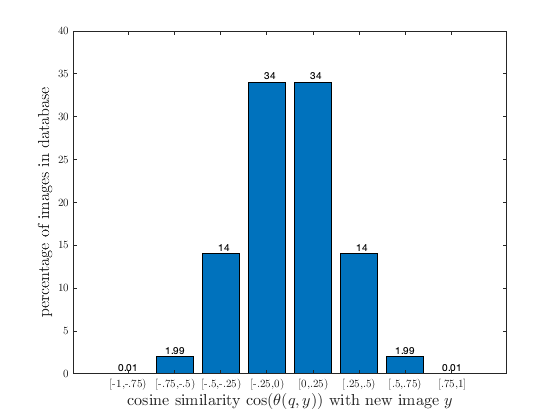
\includegraphics[width=0.65\linewidth,height=0.28\textheight,keepaspectratio]{images/problem12-figure1.png}
\end{center}

\end{document}
